% Created 2016-10-27 Thu 18:11
\documentclass[11pt]{article}
\usepackage[utf8]{inputenc}
\usepackage[T1]{fontenc}
\usepackage{fixltx2e}
\usepackage{graphicx}
\usepackage{grffile}
\usepackage{longtable}
\usepackage{wrapfig}
\usepackage{rotating}
\usepackage[normalem]{ulem}
\usepackage{amsmath}
\usepackage{textcomp}
\usepackage{amssymb}
\usepackage{capt-of}
\usepackage{hyperref}
\author{Nicholas Antonov \& Pat Grasso}
\date{\today}
\title{Homework 4}
\hypersetup{
 pdfauthor={Nicholas Antonov \& Pat Grasso},
 pdftitle={Homework 4},
 pdfkeywords={},
 pdfsubject={},
 pdfcreator={Emacs 24.5.1 (Org mode 8.3.4)}, 
 pdflang={English}}
\begin{document}

\maketitle
\tableofcontents


\section{Overview}
\label{sec:orgheadline1}

What we did was first cluster the documents. Then, for each group of documents in a cluster, we did a summation of the number of times each unique column value appeared. We then repeated this over the entire document set.

After doing this, we computed the squared distance of each cluster's average values for a column, verses the average values over the whole document set. These values show how different any cluster's makeup is from the document as a whole. We then graphed these values too see patterns, and found that the clustering does appear to be working, as different clusters have different characteristics, such as in the example submitted, cluster 2 has a very unique SPLTTYPE compared to all the other clusters

\section{Output}
\label{sec:orgheadline9}

\subsection{Graphs}
\label{sec:orgheadline7}

\subsubsection{0}
\label{sec:orgheadline2}
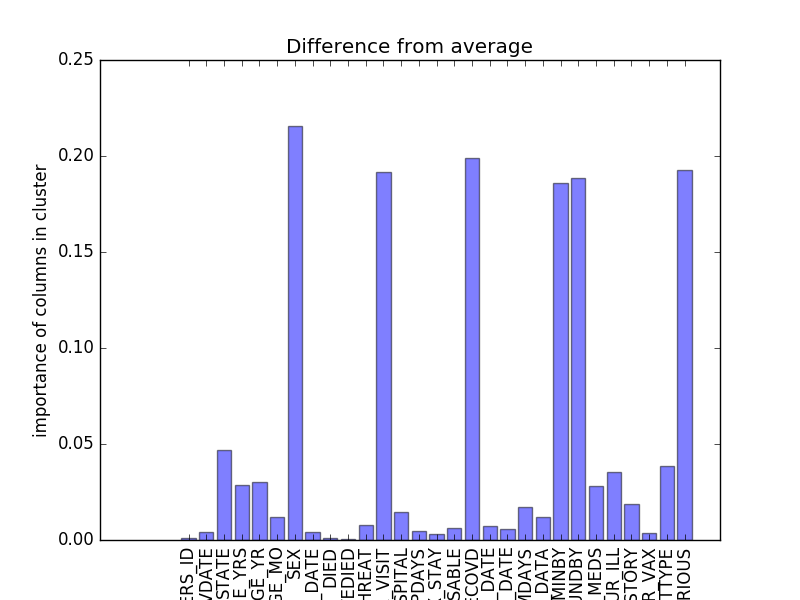
\includegraphics[width=.9\linewidth]{./cluster-weight-0.png}
\subsubsection{1}
\label{sec:orgheadline3}
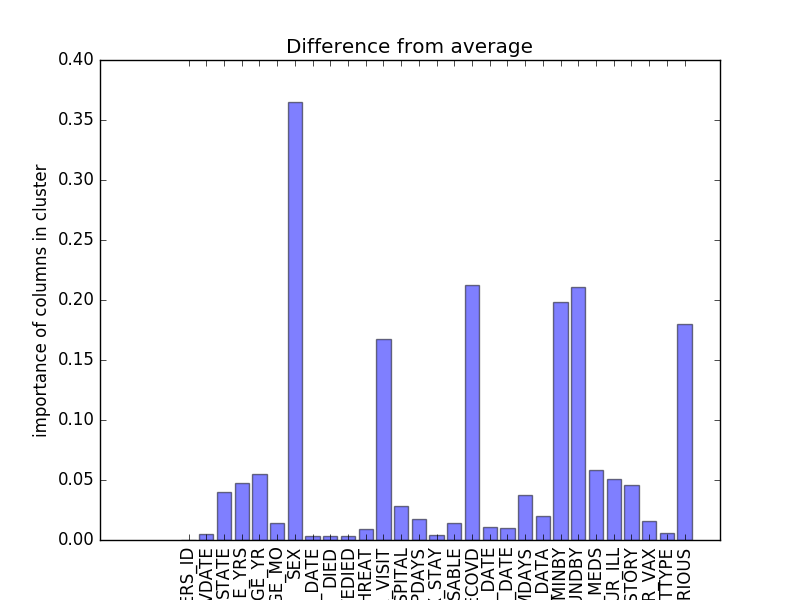
\includegraphics[width=.9\linewidth]{./cluster-weight-1.png}
\subsubsection{2}
\label{sec:orgheadline4}
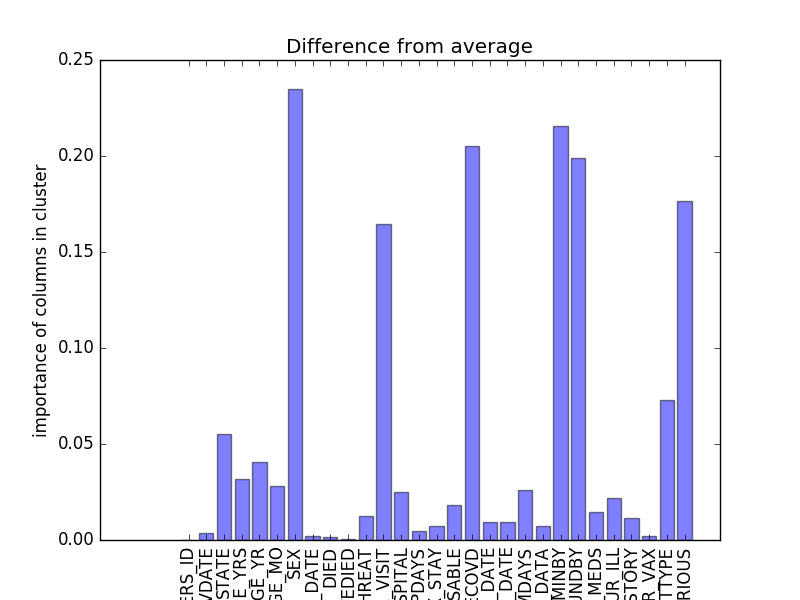
\includegraphics[width=.9\linewidth]{./cluster-weight-2.png}
\subsubsection{3}
\label{sec:orgheadline5}
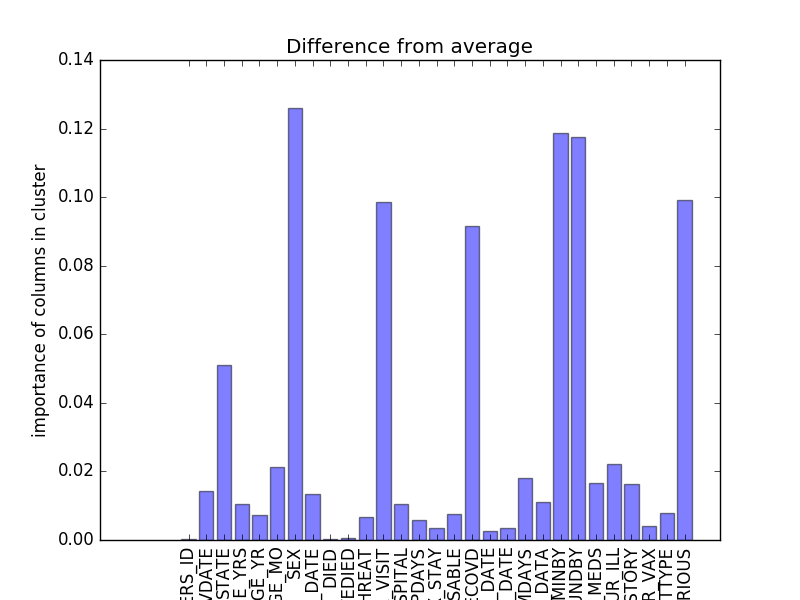
\includegraphics[width=.9\linewidth]{./cluster-weight-3.png}
\subsubsection{4}
\label{sec:orgheadline6}
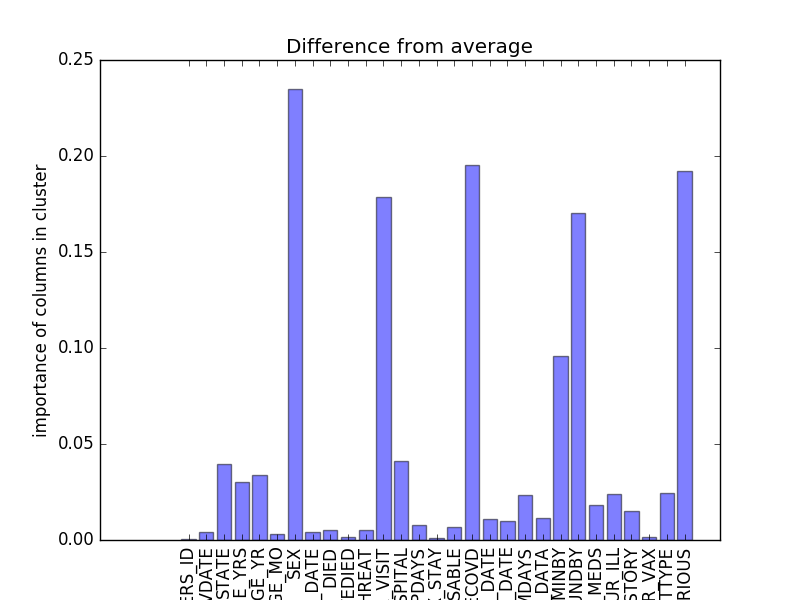
\includegraphics[width=.9\linewidth]{./cluster-weight-4.png}

\subsection{Textual}
\label{sec:orgheadline8}
\phantomsection
\label{orgexampleblock1}
\begin{verbatim}
tfidf matrix shape:
(13829, 51)
Cluster 0
Size: 1037
# serious: 423
Cluster 1
Size: 4896
# serious: 170
Cluster 2
Size: 3988
# serious: 1561
Cluster 3
Size: 2648
# serious: 307
Cluster 4
Size: 1260
# serious: 513
Segment Profile:
cluster 0
SEX 0.21582183788869094
RECOVD 0.19884222144923286
SERIOUS 0.19285210673167152
ER_VISIT 0.191547565445499
V_FUNDBY 0.18849893018113967
V_ADMINBY 0.18619691417928239
cluster 1
SEX 0.3652979722338193
RECOVD 0.21215650333589559
V_FUNDBY 0.2105062352917194
V_ADMINBY 0.19841400708750392
SERIOUS 0.18033309631129432
ER_VISIT 0.16754784867643394
cluster 2
SEX 0.23501963898679087
V_ADMINBY 0.2156288075482672
RECOVD 0.20536075236375181
V_FUNDBY 0.19879649441440214
SERIOUS 0.17636895428493882
ER_VISIT 0.16483942753127417
cluster 3
SEX 0.12599394380693987
V_ADMINBY 0.11882411816667653
V_FUNDBY 0.11745204517150949
SERIOUS 0.09911876264227788
ER_VISIT 0.09854892483700894
RECOVD 0.09144331558006305
cluster 4
SEX 0.23505336662980583
RECOVD 0.19507734197438256
SERIOUS 0.19208753860934058
ER_VISIT 0.17877568073533076
V_FUNDBY 0.1704460651124881
V_ADMINBY 0.09599558487209404
\end{verbatim}
\end{document}
